\documentclass{beamer}
\usepackage{amsmath}
\usepackage[english]{babel} %set language; note: after changing this, you need to delete all auxiliary files to recompile
\usepackage[utf8]{inputenc} %define file encoding; latin1 is the other often used option
\usepackage{csquotes} % provides context sensitive quotation facilities
\usepackage{graphicx} %allows for inserting figures
\usepackage{booktabs} % for table formatting without vertical lines
\usepackage{textcomp} % allow for example using the Euro sign with \texteuro
\usepackage{stackengine}
\usepackage{wasysym}
\usepackage{tikzsymbols}
\usepackage{textcomp}
\newcommand{\bubblethis}[2]{
        \tikz[remember picture,baseline]{\node[anchor=base,inner sep=0,outer sep=0]%
        (#1) {\underline{#1}};\node[overlay,cloud callout,callout relative pointer={(0.2cm,-0.7cm)},%
        aspect=2.5,fill=yellow!90] at ($(#1.north)+(-0.5cm,1.6cm)$) {#2};}%
    }%
\tikzset{face/.style={shape=circle,minimum size=4ex,shading=radial,outer sep=0pt,
        inner color=white!50!yellow,outer color= yellow!70!orange}}
%% Some commands to make the code easier
\newcommand{\emoticon}[1][]{%
  \node[face,#1] (emoticon) {};
  %% The eyes are fixed.
  \draw[fill=white] (-1ex,0ex) ..controls (-0.5ex,0.2ex)and(0.5ex,0.2ex)..
        (1ex,0.0ex) ..controls ( 1.5ex,1.5ex)and( 0.2ex,1.7ex)..
        (0ex,0.4ex) ..controls (-0.2ex,1.7ex)and(-1.5ex,1.5ex)..
        (-1ex,0ex)--cycle;}
\newcommand{\pupils}{
  %% standard pupils
  \fill[shift={(0.5ex,0.5ex)},rotate=80] 
       (0,0) ellipse (0.3ex and 0.15ex);
  \fill[shift={(-0.5ex,0.5ex)},rotate=100] 
       (0,0) ellipse (0.3ex and 0.15ex);}

\newcommand{\emoticonname}[1]{
  \node[below=1ex of emoticon,font=\footnotesize,
        minimum width=4cm]{#1};}
\usepackage{scalerel}
\usetikzlibrary{positioning}
\usepackage{xcolor,amssymb}
\newcommand\dangersignb[1][2ex]{%
  \scaleto{\stackengine{0.3pt}{\scalebox{1.1}[.9]{%
  \color{red}$\blacktriangle$}}{\tiny\bfseries !}{O}{c}{F}{F}{L}}{#1}%
}
\newcommand\dangersignw[1][2ex]{%
  \scaleto{\stackengine{0.3pt}{\scalebox{1.1}[.9]{%
  \color{red}$\blacktriangle$}}{\color{white}\tiny\bfseries !}{O}{c}{F}{F}{L}}{#1}%
}
\usepackage{fontawesome} % Social Icons
\usepackage{epstopdf} % allow embedding eps-figures
\usepackage{tikz} % allows drawing figures
\usepackage{amsmath,amssymb,amsthm} %advanced math facilities
\usepackage{lmodern} %uses font that support italic and bold at the same time
\usepackage{hyperref}
\usepackage{tikz}

\usepackage{tcolorbox}

\usefonttheme[onlymath]{serif} %set math font to serif ones

\definecolor{beamerblue}{rgb}{0.2,0.2,0.7} %define beamerblue color for later use

%%% defines highlight command to set text blue
\newcommand{\highlight}[1]{{\color{blue}{#1}}}


%%%%%%% commands defining backup slides so that frame numbering is correct

\newcommand{\backupbegin}{
   \newcounter{framenumberappendix}
   \setcounter{framenumberappendix}{\value{framenumber}}
}
\newcommand{\backupend}{
   \addtocounter{framenumberappendix}{-\value{framenumber}}
   \addtocounter{framenumber}{\value{framenumberappendix}}
}

%%%% end of defining backup slides

%Specify figure caption, see also http://tex.stackexchange.com/questions/155738/caption-package-not-working-with-beamer
\setbeamertemplate{caption}{\insertcaption} %redefines caption to remove label "Figure".
%\setbeamerfont{caption}{size=\scriptsize,shape=\itshape,series=\bfseries} %sets figure  caption bold and italic and makes it smaller

\newtcolorbox{boxA}{
    fontupper = \bf,
    boxrule = 1.5pt,
    colframe = black % frame color
}

\usetheme{Boadilla}

% --------------------
% Overall information
% --------------------
\title[Economía I]{Economía I \vspace{4mm}
\\ Magistral 17: Distorsiones de mercado II}
\date{}
\author[Riottini]{Riottini Franco}
\vspace{0.4cm}
\institute[]{Universidad de San Andrés} 

\begin{document}

\begin{frame}
\titlepage
\centering

\includegraphics[scale=0.2]{../Figures/logoUDESA.jpg} 
\end{frame}


\begin{frame}{Distorsiones al equilibrio de mercado}
    \begin{itemize}
        \item Por las características de la realidad.
        \begin{itemize}
            \item Monopolios naturales (red eléctrica, agua, gas)   
             \vspace{1mm}
            \item Externalidades
             \vspace{1mm}
            \item Bienes públicos
            \vspace{1mm}
            \item Problemas de información
            \begin{itemize}
                \item Atributos ocultos (selección adversa)
                 \vspace{1mm}
                \item Acciones ocultas (moral hazard o riesgo moral)
            \end{itemize}        
        \end{itemize}
    \end{itemize}
\end{frame}

\begin{frame}{Externalidades}
    \begin{itemize}
        \item Sucede cuando una decisión económica genera un beneficio o costo \textbf{externo}
        \item Afecta a terceros que no son capaces de internalizar estos beneficios o costos
        \item La clave es que estos beneficios o costos \textbf{¡no se reflejan en los precios!}
        \begin{boxA}
            \centering
            Una externalidad sucede cuando el efecto de una decisión económica genera un beneficio (o un costo) a un tercero sin que este pague o tenga que pagar por él
        \end{boxA}
        \item Dos tipos de externalidades: 
        \begin{itemize}
            \item Externalidades negativas
            \item Externalidades positivas
        \end{itemize}
    \end{itemize}
\end{frame}

\begin{frame}{Un ejemplo}
    \centering
    \href{https://econ.video/2022/06/20/the-g-word-with-adam-conover-externalities-regulation/}{
\includegraphics[scale=0.35]{../Figures/ExternalidadP.png}}  
\end{frame}

\begin{frame}{Externalidades}
    \begin{itemize}
        \item ¿Que pasa con la cantidad?
        \item ¿Como afecta esto a los productores y consumidores?
        \item ¿Como es la perdida o ganancia social?
    \end{itemize}
\end{frame}

\begin{frame}{Externalidades negativas}
    \begin{boxA}
        \centering
        Las externalidades negativas tienen lugar cuando el efecto de
        una decisión de producción, consumo u otro tipo de decisión
        económica de un agente genera un costo a un tercero que no es
        $\underline{\text{internalizado}}$ por quien lo produce.
    \end{boxA}
    \begin{itemize}
        \item La contaminación es un ejemplo clásico de externalidades negativas.
        \item El productor contaminante \textbf{no paga} por el costo extra que le está imponiendo a otros.
        \item Como no internaliza el costo "total" de su producción, produce más de lo que sería socialmente deseable.
        \item Para modelarlo, diferenciaremos entre costos marginales \textbf{privados} y costos marginales \textbf{sociales}.
    \end{itemize}
\end{frame}

\begin{frame}{Externalidades negativas}
    \begin{center}
        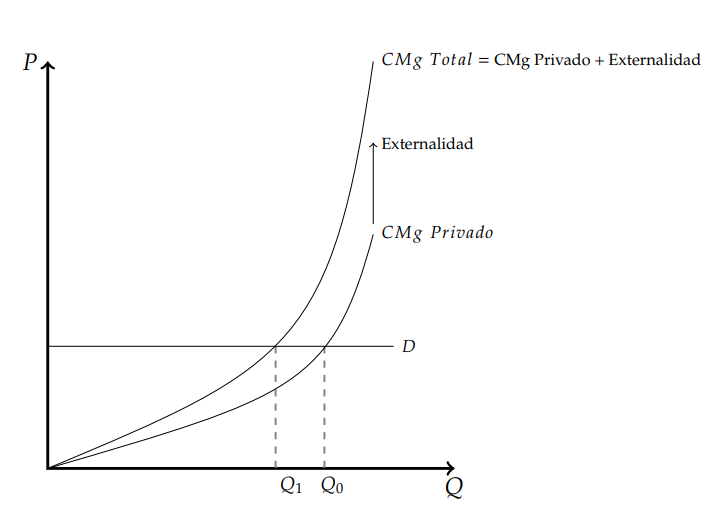
\includegraphics[scale=0.7]{../Figures/C25.2.png}
    \end{center}
\end{frame}

\begin{frame}{¿Como corregir una externalidad negativa?}
    \begin{itemize}
        \item ¿Prohibir?
        \item ¿Regular la producción o el uso del contaminante?
        \item ¿Gravar (con un impuesto) la actividad contaminante?
        \item ¿Negociación privada?
    \end{itemize}
\end{frame}

\begin{frame}{Externalidad positiva}
    \begin{boxA}
        Las externalidades positivas tienen lugar cuando el efecto de
        toda decisión de producción, consumo u otro tipo de decisión
        económica de un agente genera un beneficio sobre un tercero sin
        que este pague por él.
    \end{boxA}
    \begin{itemize}
        \item La educación es un ejemplo clásico de externalidades positivas.
        \item El individuo que se educa recibe un beneficio, pero también lo recibe la sociedad.
        \item El individuo no recibe el beneficio total de su educación, por lo que no se educa lo suficiente.
        \item Para modelarlo, diferenciaremos entre beneficios marginales \textbf{privados} y beneficios marginales \textbf{sociales}.
    \end{itemize}
\end{frame}

\begin{frame}{Otro ejemplo}
    \centering  
    \href{https://econ.video/2022/06/21/the-g-word-with-adam-conover-external-benefits-of-gps/}{
\includegraphics[scale=0.25]{../Figures/ExternalidadPII.png}}  
\end{frame}

\begin{frame}{Externalidades positivas}
    \begin{center}
        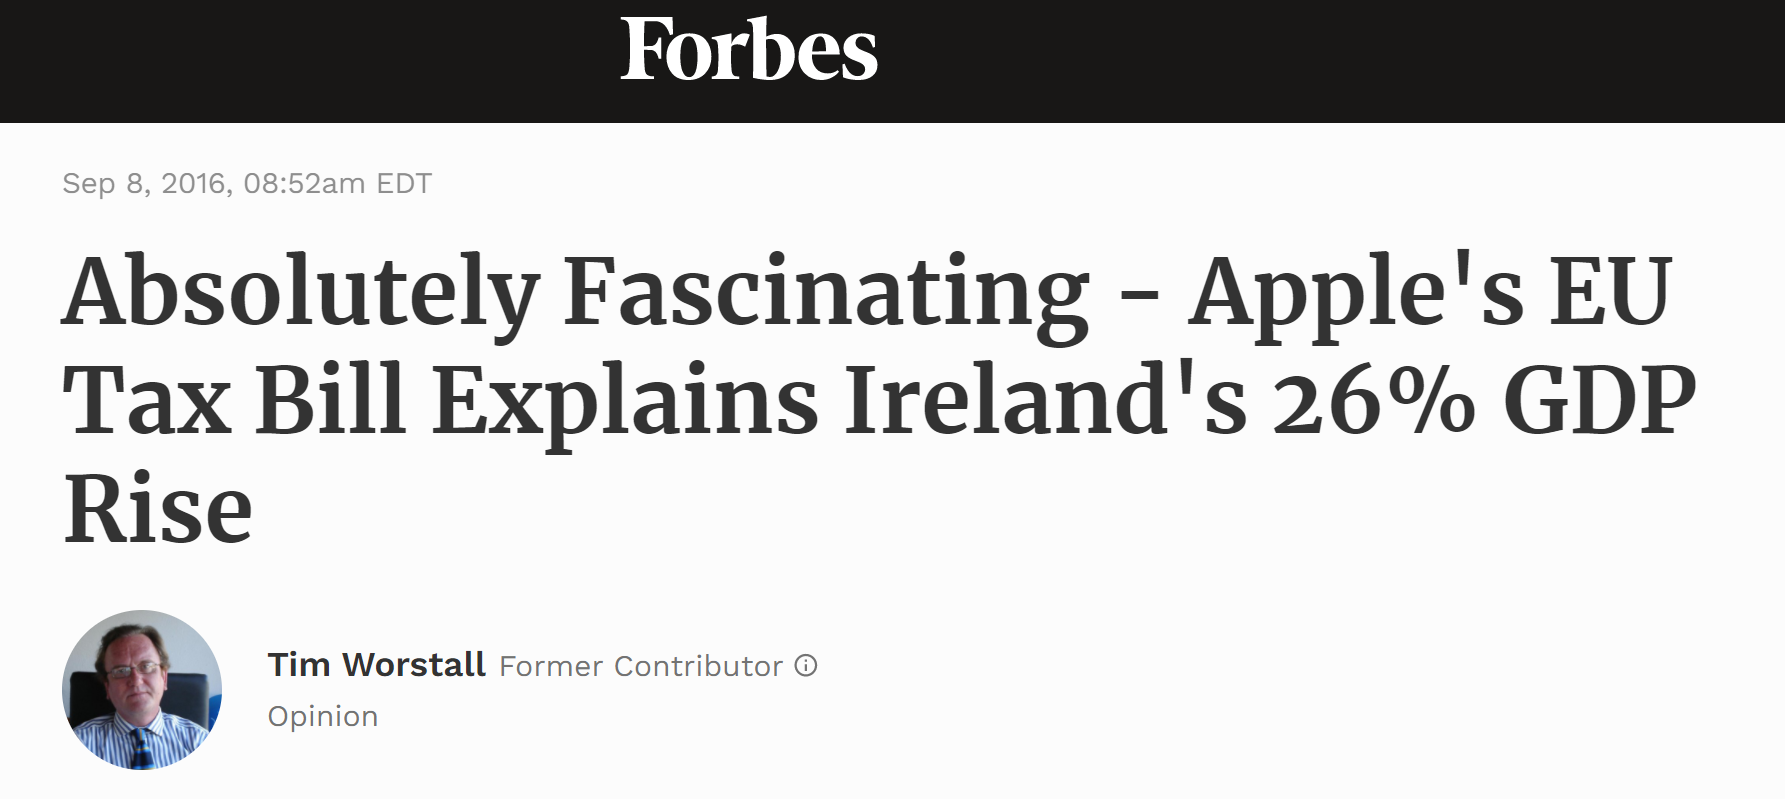
\includegraphics[scale=0.7]{../Figures/C25.1.png}
    \end{center}
\end{frame}

\begin{frame}{¿Qué hacer con las externalidades positivas?}
    \begin{itemize}
        \item ¿Obligar?
        \item ¿Subsidiar su consumo?
    \end{itemize}
\end{frame}

\begin{frame}{Teorema de Coase}
    \begin{itemize}
        \item Coase dice que las externalidades no son un problema
        \item ... si los derechos de propiedad están bien definidos y los costos de transacción son nulos
        \item Esto es así porque ``hay una ganancia para apropiar'' de buscar un óptimo 
    \end{itemize}
    \begin{boxA}
        \centering
        El Teorema de Coase señala que, en ausencia de costos de transacción y con derechos de propiedad bien definidos, una negociación
        entre las partes puede resultar en una asignación de recursos
        Pareto Eficiente, sin la necesidad de la intervención del Estado.
    \end{boxA}
\end{frame}

\begin{frame}{Coase I}
    \begin{center}
        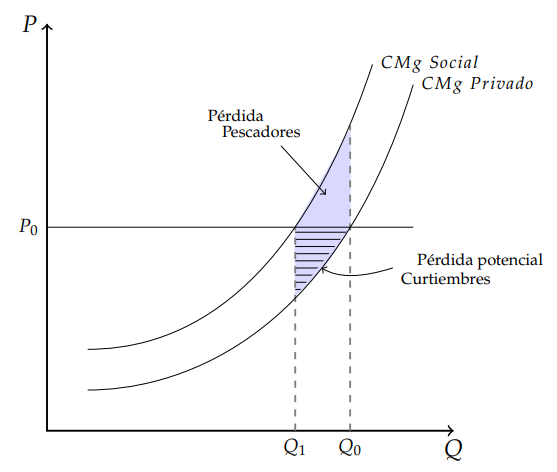
\includegraphics[scale=0.7]{../Figures/C25.6.png}
    \end{center}
\end{frame}
 
\begin{frame}{Coase II}
    \begin{center}
        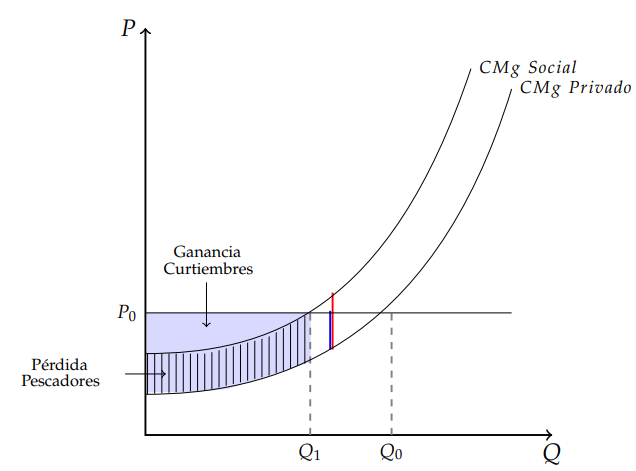
\includegraphics[scale=0.7]{../Figures/C25.7.png}
    \end{center}
\end{frame}

\begin{frame}{Bienes Públicos}
    \begin{itemize}
        \item Vamos a distinguir los bienes por dos características
        \begin{itemize}
            \item Si su consumo es rival: ¿El consumo de un individuo impide que otro lo consuma?
            \item Si su consumo es excluible: ¿Es posible impedir que alguien consuma el bien en base a algun criterio?
        \end{itemize}
        \item Estas características hacen que los bienes divergan de los que conocemos como \textbf{bienes privados}.
        \item Los bienes públicos son no rivales y no excluibles: ¿Por qué no los puede ofrecer el mercado?
    \end{itemize}
    \begin{table}[]
        \centering
        \begin{tabular}{|c|c|c|}
    \hline
                        & \textbf{Rival}   & \textbf{No rival} \\ \hline
    \textbf{Excluible}    & \textbf{Bienes privados}  & Bienes club       \\ \hline
    \textbf{No Excluible} & Recursos comunes & \textbf{Bienes públicos}   \\ \hline
    \end{tabular}
    \end{table}
\end{frame}

\begin{frame}{Bienes Club}
    \centering
    
\includegraphics[scale=0.5]{../Figures/derechos_autor.png}
    
\includegraphics[scale=0.5]{../Figures/Escudo_del_C_A_River_Plate.png}
\end{frame}

\begin{frame}{Bienes Comunales}
    \begin{boxA}
        \centering
        La tragedia de los comunes describe la situación en la que los individuos acaban sobreexplotando los recursos comunes puesto que,
        como se trata de bienes rivales y no excluibles, tienen incentivos
        para utilizarlos antes que el resto.
    \end{boxA}
    \centering
    
\includegraphics[scale=0.7]{../Figures/socialismo.png}
\end{frame}

\end{document}
